\chapter{Plugin továbbfejlesztése}

Ebben a fejezetben ismertetem a beépülő modulon végzett továbbfejlesztéseket. Kezdetben bemutatom a fejlesztés céljait ezt követően ismertetem, hogy ezeket hogyan valósítottam meg. Bemutatom a feladat elvégzése során készített UML profilt és ennek elemeit illetve azt, hogyan valósítottam meg a kompozíció leképzését ennek segítségével. Ezt követően emutatom milyen megoldást alkalmaztam a modellen ellenőrizendő tulajdonságok megfogalmazására. Kitérek a plugin validációs szabályaira és elmagyarázom miért van szükség rájuk, végül rövid példán bemutatom az elkészült funkciók használatát.

\section{Fejlesztés céljai}

A fejlesztés során alkalmazott megoldások áttekintése előtt érdemes végigvenni, hogy mik is voltak a fejlesztés fő céljai és mi volt ezeknek a motivációja.

\subsection{Kompozit állapotgép definíciók támogatása}
Egy rendszert állapotait és állapotváltásait le lehetne modellezni egy mindent tartalmazó állapotgéppel, párhuzamos régiókkal és egyéb modellezési megoldásokkal. Ahogy a modell mérete nő a funkcionalitást érdemes feldarabolni és részenként modellezni. Ez nem csak az áttekinthetőséget segíti, de megkönnyíti a modellen való csapatmunkát is a mérnökök számára hiszen a szétbontott részeket külön, egymástól független lehet modellezni, majd ezeket összekapcsolni.

Szerencsére a Gamma erre a problémára is megoldást kínál, támogatja állapotgépek kompozíciójának modellezését és formális verifikációját. A fejlesztés egyik fő célja modell alapú kompozit rendszerek modellezésének és transzformációjának támogatása MagicDraw - SysML modellek esetében.

\subsection{Eredmények megjelenítése}
Fontos kérdés, hogy a formális verifikáció eredményét milyen formában kívánjuk megjeleníteni a mérnökök számára. A plugin korábbi verziója csak arra a kérdésre tudott választ adni, hogy teljesülnek-e a modellel szemben támasztott megkötések vagy sem.

Az \uppaal\ és a Gamma is képes sokkal részletesebb választ adni. Ezt a Gamma \emph{back-annotation} formájában teszi azaz a verifikációban előállt időzítések és lépéseket visszavezeti az eredeti modellbe. Ehhez a Gamma egy elég jól értelmezhető nyelvtant definiál, azonban a SysML-t jellemzően rendszermérnökök használják akik általában a szöveges leírások helyett a diagramokat preferálják.

A modellbe visszavezetett lépések, \emph{trace}k, a modell egy futtatását írják le. Ezek szinkron esetben egymástól jól elkülönülő lépés sorozatok. Ezt leginkább szekvencia diagramokon lehet ábrázolni. További érv a szekvencia diagramok alkalmazása mellett az a MagicDraw, illetve a Cameo Simulation toolkit. Ez ugyanis lehetőséget biztosít szimulációk rögzítésére szekvencia diagramok formájában (\refstruc{fig:md-cameo-rec})) melyekkel a futtatás elméletben reprodukálható. A cél tehát olyan szekvencia diagramok előállítása úgy minthogyha a szimulátort használva találtuk volna meg a hibautakat, így ezekről nem csak egy jól áttekinthető megoldást kapunk szekvenciák formájában, hanem ezek akár szimulálhatóak is lehetnek Cameo Simulation Toolkit segítségével.

%TODO kisebbre
\begin{figure}[!ht]
	\centering
	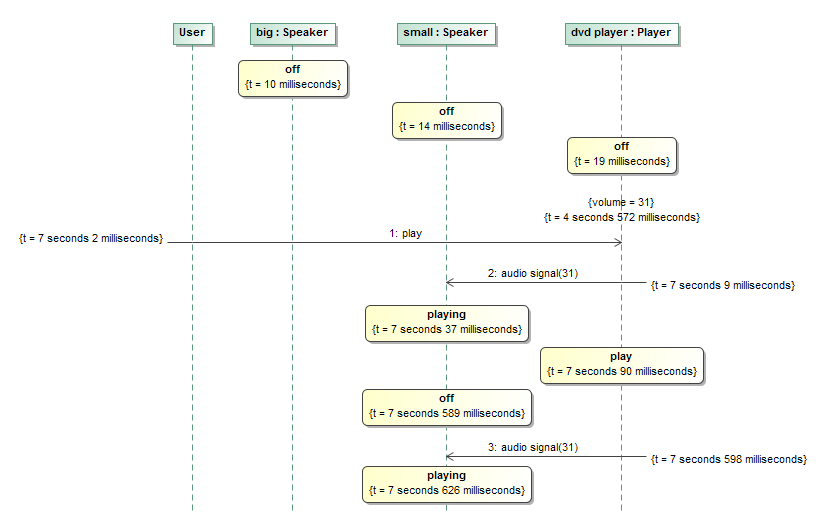
\includegraphics[width=120mm, keepaspectratio]{figures/contribution/md-cameo-rec.png}
	\caption[]{Rögzített szimuláció szekvencia diagramon\footnotemark}
	\label{fig:md-cameo-rec}
\end{figure}

\footnotetext{Forrás: https://docs.nomagic.com/display/CSTD184/Recording+simulation+as+a+Sequence+diagram}

\subsection{Követelmények definiálása}

A formális verifikáció elvégzéséhez a modelleken felül meg kell tudnia a felhasználónak azokat a kérdéseket melyekre választ szeretne kapni a modell ellenőrzése során. Ezek jelen esetben a "Kerülhet-e a rendszer adott állapotba" illetve "Adott állapotból el tud-e jutni egy másikba" típusúak lehetnek. Az \uppaal-ban ezeket temporális logikai kifejezések segítségével tudjuk megtenni \uppaal Queryk formájában ezért ezeket az ellenőrzés során elő kell állítanunk.

A Gammához készült egy úgynevezett \emph{Property Language} és ez ennek az \uppaal-ra transzformáló funkciója és ezt terveztem felhasználni. Ez szintén temporális logikai kifejezéseket ír le viszont nem az \uppaal\ bemenetét képező időzített automatákon hanem magukon az állapotgépeken.

\subsection{Validáció}

A fejlesztés során hozott számos döntés megköveteli, hogy a modellekre vonatkozzanak bizonyos jól-formáltsági kényszerek. Ezek egy része a Gammából örökölt. Például a \emph{Property Language} egy komponensen belül egy állapotra a régión keresztül tudunk hivatkozni (\emph{[component]+.region.state}). Ebből következik, hogy a régióknak a MagicDraw modellben nevet kell adni, illetve, hogy ezek egyediek legyenek egy állapottérképen belül.

A munkám egyik célja egy validációs szabálykészlet létrehozása ami segít a felhasználóknak az eszköz helyes használatában.

\newpage

\section{Gamma UML profil}

A dolgozat elkészítéséhez pusztán a SysML nyelv nem volt elegendő ugyanis szükséges volt  a modellben is eltárolni  bizonyos információkat, mint például az ellenőrizendő követelmények, a  \emph{back-annotation}, vagy éppen, hogy milyen kompozit szemantikát kívánunk érvényesíteni az adott modellekre. Ezt többféleképpen meg lehet valósítani például speciális nevezéktannal, én viszont egy UML profil készítése mellett döntöttem. Ez lehetővé teszi, hogy az egyes elemeket könnyebb legyen keresni és nagyobb flexibilitást is ad például saját mezőket tudtam definiálni amik akár lehetnek származtatottak is. Az elemeknek továbbá megkötéseket tudok előírni a tartalmazási hierarchiára.

Az UML három részből áll:

\begin{itemize}
	\item Kompozit szemantika
	\item Check modell
	\item Back-annotation modell
\end{itemize}

Az UML profil érdekessége, hogy tartalmazásokat csak megkötés szintjén \emph{Customization}on keresztül tudunk megadni. UML profil diagramon csak öröklést és \emph{tag}eket van lehetőségünk definiálni.

\subsection{Kompozit szemantika}

A Gamma háromféle komponens végrehajtási szemantikát biztosít a felhasználók számára. Ugyan ezt implicit módon is meg lehet határozni, például a kommunikáció típusából, mégis fontos lehet ezek egyértelmű jelölése. Ezért az UML profil (\refstruc{fig:comp-prof}) a SysML nyelvet kiegészíti néhány sztereotípiával melyek segítségével explicit jelölhetők, hogy milyen szemantikát szeretne a felhasználó érteni Blokkjain.

\begin{figure}[!ht]
	\centering
	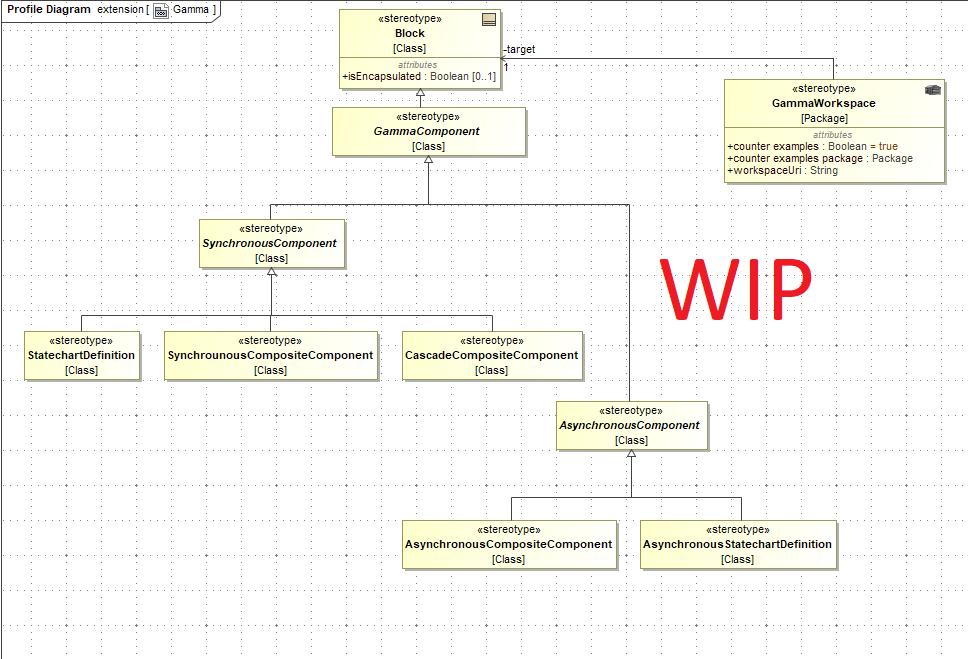
\includegraphics[width=130mm, keepaspectratio]{figures/contribution/profile.png}
	\caption{Szinkron, asszinkron szemantikát támogató UML profil}
	\label{fig:comp-prof}
\end{figure}

A sztereotípiák leszármaznak a Block sztereotípiájából, így lényegében lecserélik azt. Ennek előnye hogy szintaktikailag is asszinkron és szinkron blokkok fognak megjelenni a modelljeinkben. Viszont van egy nagy hátránya is mégpedig az, hogyha már meglévő modelleken szeretnénk használni az eszközt szükség van azok módosítására, amire nem mindig van lehetőség, például elosztott környezetben. Sokszor azonban az őrfeltételekre, akciókra és interfészekre vonatkozó megkötések már önmagukban megkövetelik a modellek módosítását, hiszen ezek nagy valószínűséggel nem a támogatott módszertant követik.

Egy alternatív megoldás az lehetne, hogy a sztereotípiákat valamilyen él például \emph{Dependency} segítségével rendeljük az egyes komponens definíciókhoz, vagy komponensekhez, \emph{part}okhoz. Ez megoldást nyújthat arra a problémára is, hogyha a modell egyes részei külső könyvtárból jönnek, vagy nincs hozzáférésünk hozzájuk.


\subsection{Check modell}

Ahhoz, hogy a formális verifikáció végrehajtható legyen ki kell választani, hogy milyen modelleket szeretnénk ellenőrizni és ezeken milyen követelményeket. Az formális verifikációt modell elemeken keresztül lehet paraméterezni.

Az elképzelés szerint a felhasználó \emph{Workspace}eket hoz létre. Ezek hivatkoznak a felhasználó számítógépén egy könyvtárra melyet az infrastruktúra sajátosságából adódó háttértárra kimentendő modelleket tárolására használok. Ezen felül rajta keresztül kell behivatkozni az ellenőrizendő modellt a projektből.

A modell transzformációk során \emph{Trace}k keletkeznek. Ezek alapján lehet visszakeresni, hogy a MagicDraw - Gamma transzformáció során milyen leképzések történtek. Ezek valójában UML propertyk egy \emph{Class}on belül melyeknek a neve egy azonosító amivel a Gamma modell egy kisorosított XMI fájlban lévő elemei vannak hivatkozva. A \emph{property}kből egy \emph{Trace} él mutat a megfelelő MagicDraw elemekre. A kisorosított XMI-k ugyanezen \emph{Class}okhoz \emph{Comment} formájában vannak hozzárendelve, innen lehet őket kiolvasni.

A követelményeket \emph{GammaProperty} segítségével lehet megadni a Gamma által definiált Property nyelvtan segítségével. Az ezek ellenőrzéséből származó Back-annotaion modellek is a \emph{Workspace}ben helyezkednek el. A modell elemei a következők (\ref{fig:Infrastructure} ábra):

\begin{figure}[!ht]
	\centering
	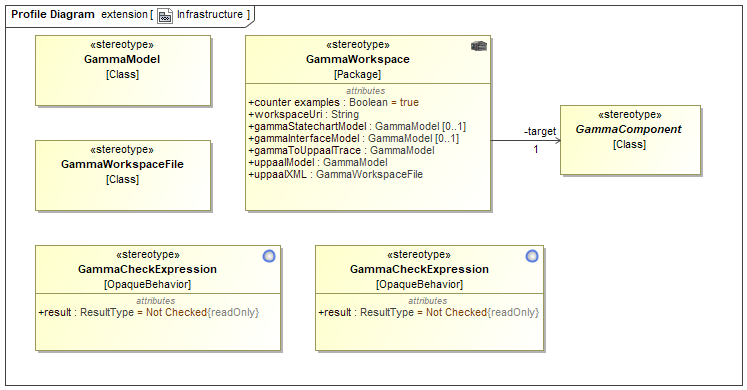
\includegraphics[width=120mm, keepaspectratio]{figures/contribution/Infrastructure.png}
	\caption{Infrastruktúra elemei}
	\label{fig:Infrastructure}
\end{figure}


\begin{itemize}
	\item \textbf{GammaWorkspace} \newline
	Letranszformált modellek és egyéb konfigurációkat és köztes állapotokat tároló modell eleme a projektben.
	
	Ennek az elemnek három fontos attribútuma van. A \emph{Target: Block[1]} kijelöli azt a blokkot amin a funkcionalitás végre szeretnénk hajtani. A \emph{WorkspaceUri: String[1]} ami kijelöl egy könyvtárat a háttértáron, hogy oda sorosodjanak ki azok a modellek amiket az UPPAAL fog használni a futtatás során. Azt, hogy szernénk-e vissza annotálni az ellenpéldát a modellben a \emph{Counter example: Boolean[1]} állításával tudjuk megadni. Ezeken kívül még referenciákat is tárol a majdani letranszformált modellekre.
	
	\item \textbf{GammaCheckExpression} \newline
	Egy \emph{Opaque Behavior} ami a törzsében(\emph{body}) a Gamma \emph{Property Language} segítségével definiált tulajdonságokat tárol a modellre vonatkozóan. Itt fontos megjegyezni, hogy ezekben az elemekben nyelvet is lehet specifikálni. Ezt viszont figyelmen kívül hagytam és mindenképp az előbbi nyelvtan szerint értelmezem a kifejezéseket.

	\item \textbf{GammaModel} \newline
	Letranszformált Gamma modelleket tárol XMI-k formájában az elemhez csatolva kommentként. Ezen kívül \emph{property} elemeket tartalmaz amelyek a Gamma - MagicDraw visszakereshetőségért felelnek a következőképp: a MagicDraw elemre egy Trace él mutat a \emph{property}ből, a Gammabeli modell elem pedig EMF hivatkozás formájában kerül tárolásra mint az elem neve.
	

	\item \textbf{GammaWorkspaceFile} \newline
	Hivatkozás egy Gamma modellre a háttértáron. A modell elem neve a fájl elérési útja.
	
\end{itemize}

\subsection{Back-annotation modell}
A back-annotation modell feladata visszacsatolni az eredeti modellbe a valamilyen külső, jellemzően szimulátorból származó időzítési adatokat. A Gamma is készít egy ilyen modellt. A megoldás amit kidolgoztam Gamma modell egy MagicDraw specifikus változatának létrehozásából és egy Gamma-MagicDraw transzformáció megtervezéséből és megvalósításából állt. Az UML profil egy szakterület specifikus nyelvet definiál. Elemei pedig a következők:

\begin{figure}[!ht]
	\centering
	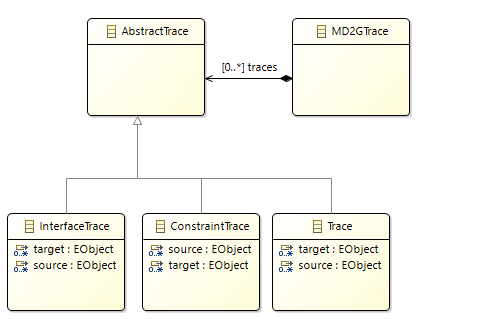
\includegraphics[width=90mm, keepaspectratio]{figures/contribution/trace-model.png}
	\caption{Back-annotation UML profilja}
	\label{fig:contribution-trace-profile}
\end{figure}

\begin{itemize}
	\item \textbf{ExecutionTrace} \newline
	Egy kompozit komponens végrehajtásának menetét rögzíti. A végrehajtás \emph{Step}ekből illetve a végrehajtás végén egy ciklusból állhat. A ciklus pedig további \emph{Step}ekből. Az \emph{ExecutionTrace} egy hivatkozást is tárol az adott komponensre.
	
	\item \textbf{Step} \newline
	A végrehajtás egy lépése. Ez három részből áll. Az elsőben leírja, hogy milyen állapotokat vettek fel a komponensek és milyen értékeken álltak a változók. A másodikban, hogy mely események érkeztek és vezetnek át majd a következő lépésbe. A harmadik rész pedig a kimenő eseményeket rögzíti. 
	
	\item \textbf{Act} \newline
	Absztrakt sztereotípia. Egy végrehajtott művelet.
	
	\item \textbf{ComponentSchedule} \newline
	Komponensen egy kör végrehajtása (üzenetek kiolvasása az üzenetsorokból, állapotok léptetése)
	
	\item \textbf{TimeElapse} \newline
	Várakozást, az idő múlását szimbolizálja. Ez az érték milliszekundumban egész számként van megadva az elem \emph{Value} mezőjében.
	
	\item \textbf{RaiseEventAct} \newline
	Egy esemény elküldése a komponens példánynak. Egy \emph{Activiy} diagramot tartalmazó \emph{Class}. Ez a diagram az adott szignált küldő egyetlen akcióból áll.
	
	\item \textbf{InstanceState} \newline
	Absztrakt. Az egyes példányok, partok állapotainak leírása. Itt tárolódik a referencia arra a \emph{Part}ra amelyiknek az állapotai rögzítésre kerülnek.
	
	\item \textbf{InstanceVariableState} \newline
	Egy változónak adott lépésben felvett értékét tárolja.
	
	\item \textbf{InstanceStateConstant} \newline
	Az tárolja, hogy adott lépésen belül milyen állapotban volt a \emph{Part}.
\end{itemize}


\newpage
\section{Kompozíciók transzformációja}

Egy nagy komplex rendszert célszerű nem egyben, hanem részekre bontva modellezni majd a részek egymáshoz illesztéséből, komponálásából képezni a teljes rendszert. Állapottérképek dekomponálását azaz részekre bontását a Gamma is támogatja. A kihívás a SysML és a Gamma közötti megfeleltetések megválasztása oly módon, hogy a szemantika ne sérüljön. A megfeleltetés két szempontól kell vizsgálni, egyszer az elemek tartalmazási hierarchiái szerint, egyszer pedig a köztük modellezett kommunikáció szerint.

\subsection{Struktúra megfeleltetése}
A Gammában nyelvi szinten elkülönül az állapottérkép (StatechartDefinition) és a kompozit komponens (Composite Component) fogalma. Állapottérképek a modell hierarchia gráfjában a levelekben helyezkednek el. SysML esetében a minden Blokknak lehet viselkedése, jelen esetben állapottérképe. A megfeleltetés elvégzéséhez megkötést fogalmaztam meg amely szerint kétféle blokk megengedett meg.\\
\begin{itemize}
	\item a viselkedéssel rendelkezőket, amelyek nem tartalmaznak \emph{Part}okat
\end{itemize}
és
\begin{itemize}
	\item a viselkedés nélkülieket, melyek \emph{Part}okat tartalmaznak.\\
\end{itemize}
Előbbiek a tartalmazási hierarchiában a levél elemek. Ezzel a módszerrel nem fordulhat elő, hogy egy Blokknak nem egyértelmű a viselkedése. Hiszen ezt mindig a tartalmazottjai adják. Fontos, hogy csak olyan modelleket lehet ellenőrizni amik legalább egy \emph{Part}ot tartalmaznak. Azaz a legkisebb modellnek állnia kell legalább két blokk definícióból amelyek a két már fent említett esetek egyikébe esnek.

\begin{figure}[!ht]
	\centering
	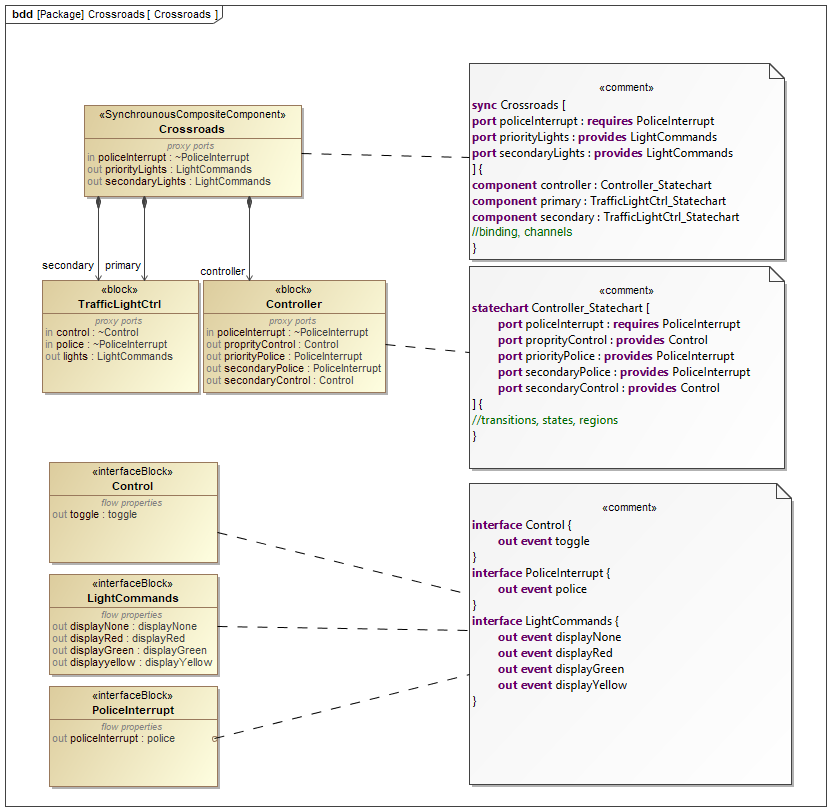
\includegraphics[width=140mm, keepaspectratio]{figures/contribution/md2g.png}
	\caption{Struktúra megfeleltetése}
	\label{fig:md2g}
\end{figure}

Az érdekes kérdés lehet, hogy ha egy magasabb szintű blokknak mégis lehetne viselkedése, azt szemantikailag hogyan kezelhetnénk. Elképzelhető olyan értelmezés, hogy ez a magas szintű állapottérkép a dekomponált részek együttes viselkedését írja le. Ez lehetőséget adna arra, hogy a magasabb és az alacsonyabb szintű viselkedés halmazt összehasonlítsuk működés szempontjából és ha nincsenek szinkronban akkor tervezési hibaként értelmezzük. Így a magasabb hierarchia szintek tulajdonképpen validálnák az alacsonyabb szinteket. Ennek a lehetőségnek a komolyabb kifejtése azonban nem célja a dolgozatnak.

\subsection{Kommunikáció megfeleltetése}

A Gammában a komponensek kommunikációja kimondottan az eseményvezérelt állapot alapú rendszerek sajátosságain alapul, azonban SysML-ben a kommunikáció leírása sokkal általánosabb és többféle módon is modellezhető. Éppen ezért a feladat elvégzése során az események és az interfészek modellezésére megkötéseket kellett megfogalmazni.
Az egyik ilyen megkötés szerint a portoknak interfész blokkokkal kell, hogy tipizálva legyenek.

Az eseményeknek mindig specifikálniuk kell, hogy melyik porton várják a szignál érkezését. Ez igaz az akciókra is. Az ő esetükben azt kell specifikálni, hogy milyen porton keresztül történjen a küldés.

Portok közül csak a \emph{Proxy} portok támogatottak. Ennek oka, hogy talán ezek állnak legközelebb a Gammában használatos portokhoz szemantikailag szemben például a \emph{Full Port}okkal. Utóbbiak a rendszer külön részeinek tekinthetők és saját tulajdonságokkal bírhatnak, míg a \emph{Proxy} portok a blokkjuk tulajdonságaihoz nyújtanak hozzáférési pontot a "külvilágnak". Azt, hogy melyek pontosan ezek a tulajdonságok az \emph{Interface Block} definiálja.
A Proxy portok iránya származtatott a \emph{Flow property} irányokból amik keresztül mehetnek rajta. Az irány az \emph{isConjugated} flag igazra állításával változtatható.

\section{Modell tulajdonságainak leírása}

A modell felett meg kell tudnunk fogalmazni tulajdonságokat, amelyeknek a teljesülését formális verifikáció segítségével szeretnénk majd igazolni. Ezeknek a tulajdonságoknak sokféle módon le lehetne írni, például Object Constranint Language (OCL) segítségével, esetleg valamilyen szcenárió alapú leírással. A Gamma esetében lehetősége van a felhasználóknak elágazó idejű tempóralis logikai kifejezésekkel tulajdonságokat megfogalmazni (példa: \ref{fig:ctl} ábra). A feladat elkészítéséhez ezt a nyelvtant használtam fel.

Az elágazó idejűség azt jelenti, hogy a rendszernek nem csak egy,  hanem az összes lefutását vizsgáljuk egyszerre. Éppen ezért meg kell tudnunk mondani azt, hogy egy tulajdonság teljesülését minden lefutás esetében elvárunk, vagy megelégszünk azzal, hogy van olyan lefutás ahol teljesül. Ezek jelölése a nyelvben az "A" (for all futures) és az "E" (exits future) kvantorok.

Az egyes útvonalakon is meg kell tudnunk mondani, hogy a tulajdonság teljesülését mikor várjuk. Valamikor a jövőben vagy esetleg minden lépésben azaz a tulajdonság invariáns. Ezek jelölései az "F" (future) és a "G" (globally). A nyelv ezeken felül támogatja még az "X" (next), "U" (until) és "R" (release) operátorokat is.

\begin{figure}[!ht]
	\centering
	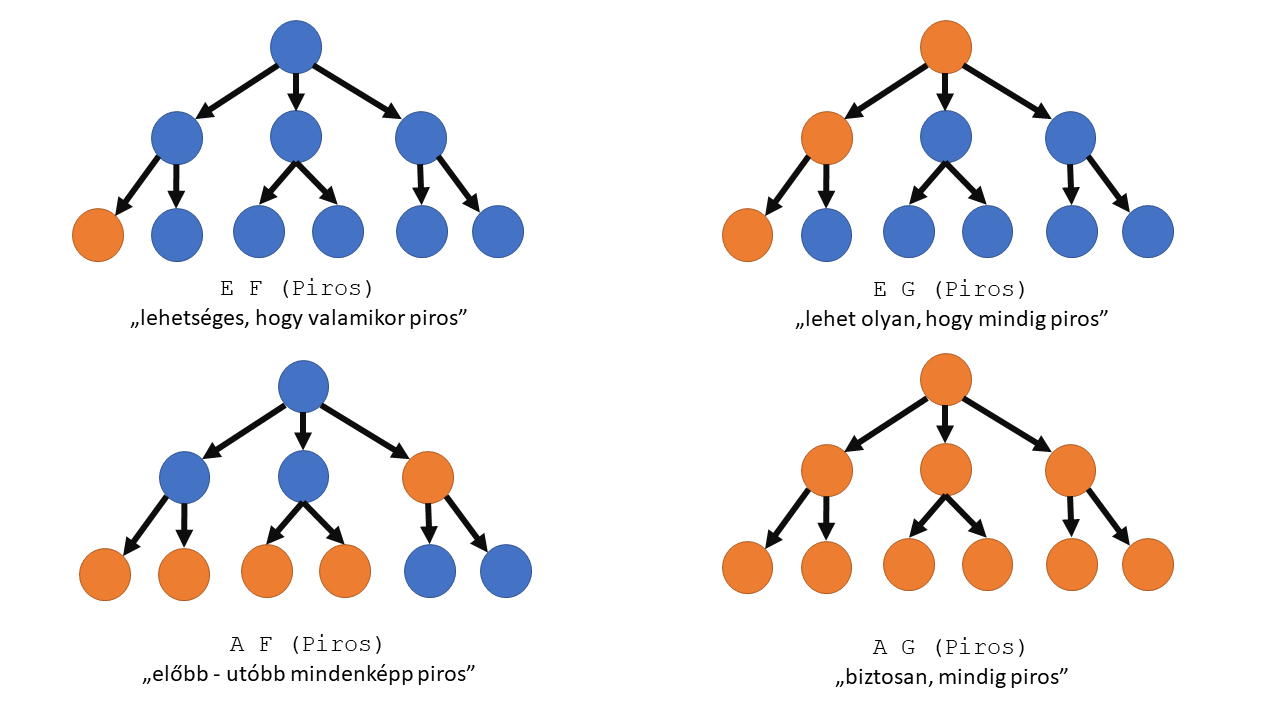
\includegraphics[width=140mm, keepaspectratio]{figures/contribution/CTL.png}
	\caption{Példa: CTL kifejezések}
	\label{fig:ctl}
\end{figure}

\subsection{Kifejezések a definiálása és használata}
A modellben a kifejezéseket \emph{Check Expression}ök törzsében kell megadni. Ezeknek a modell elemeknek egy tetszőleges \emph{package}ben kell lennie aminek viszont egy \emph{GammaWorkspace}ben. Ellenőrzés során a kifejezések kiolvasásra kerülnek és Xtext segítségével \emph{parse}oldónak. Fontos, hogy ez a nyelvtan Gamma modellekre képes hivatkozni nevezetesen állapotokra és változókra, éppen ezért el kell végezni a MagicDraw - Gamma transzformációt mielőtt a \emph{parse}olást elvégeznénk. A transzformáció után a hivatkozható elemek ugyanazon a néven szerepelnek és ugyan olyan hierarchiában a két modellben ezért nem volt szükséges a kettőt objektum szinten is összekapcsolni. Ez  a kérdés azért fontos mert ezeket a tulajdonságokat a SysML modellen és nem pedig a Gamma modellen szeretnénk kimondani.

Érdemes megjegyezni, hogy mivel a Gamma a háttérben az \uppaal\ segítségével végzi a formális verifikációt ezeket a kifejezéseket még át kell alakítani UPPAAL queryvé. Ezt a konverziót a Gamma elvégzi. Igazából ez az a lépés ahol a Gamma modellek megléte szükségessé válik, hiszen az állapot és változó neveknek a majdani \uppaal\ modellben is helyesnek kell lenni.


\section{MagicDraw modellek back-annotációja}

Bizonyos tulajdonságok meglétét vagy éppenséggel hiányát ellenpéldák igazolják. Ezeket a Gamma back-annotation segítségével vezeti vissza az ellenőrzött modelljeibe. A fentebb ismertetett UML profilt azért hoztam létre, hogy ezeket az ellenpéldák, vagy hibautak könnyebben modellezhetőek legyenek.

Ezeknek az előállítása most is modell transzformációkon keresztül történik, azonban ezek iránya itt megfordul nem MagicDraw modellekből állítok elő Gamma modelleket hanem épp fordítva Gamma modelleket transzformálok MagicDraw modellekké. Egyébként erre a modellre nem feltétlenül lenne szükség hiszen a további származtatásokat már a Gamma modellek segítéségével is meg lehetne valósítani. Viszont a végrehajtás íj módon történő tárolása már nem függ a Gammától és általánosabb mint egy \emph{activiy} diagram vagy egy szekvencia, ezért könnyebb bemenetként használni olyan transzformációkhoz ami ezeket állítja elő, esetleg valami dokumentációt generál.

\begin{figure}[!ht]
	\centering
	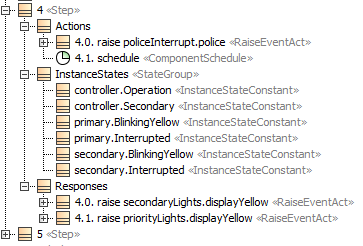
\includegraphics[width=90mm, keepaspectratio]{figures/contribution/steps.png}
	\caption{Lépések felbontása}
	\label{fig:steps}
\end{figure}

Egy ellenpélda lépéseket ír le amik a feltétel sérüléséhez vezetnek (\ref{fig:steps}). A lépések rögzítik az aktuális állapotot, az akciókat amik a következő lépésbe vezetnek és a kimeneti eseményeket.
Az lépések közti akciók és a kimenet \emph{Activiy} diagramokra képződnek le. Ezek jellemzően egy akciót tartalmaznak például egy szignál küldést ami az őt tartalmazó osztály egy portján keresztül küld eseményeket. Ez azért jó mert így a rendszerünkből létre tudunk hozni egy \emph{Part}ot amire ha rákötünk egy ezekből a \emph{RaiseEvent}ekből leszármazó blokkal tipizált partot akkor ez képes lesz kommunikálni a rendszerünkkel (\ref{fig:trace-signals} ábra).

\begin{figure}[!ht]
	\centering
	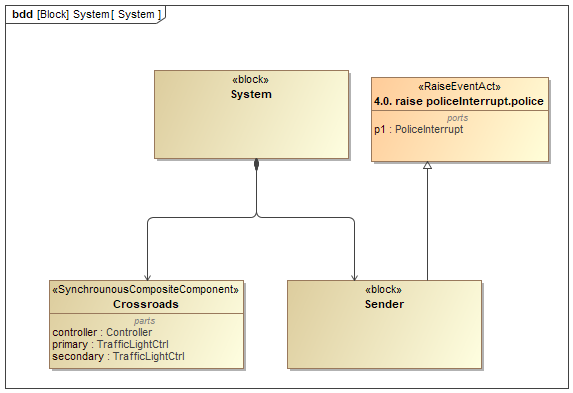
\includegraphics[width=110mm, keepaspectratio]{figures/contribution/trace1.png}
	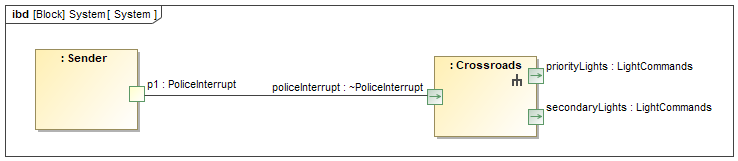
\includegraphics[width=110mm, keepaspectratio]{figures/contribution/trace2.png}
	\caption{Üzenetek küldése a rendszernek}
	\label{fig:trace-signals}
\end{figure}


\newpage\section{Szimuláció}

A fejlesztés során igyekeztem olyan modelleket előállítani amik az példákat írják le és szimulálhatók. Ez sajnos részben a szimulációs eszköz képességei miatt nem tudott maradéktalanul megvalósulni, viszont az előállított modellek pontosabban az őket ábrázoló diagramok mint megjelenítési formák egészen ígéretesnek bizonyultak. Továbbá esetleg később ahogy fejlődik a szimulációs eszköz lehetséges, hogy kis alakításokkal lehetővé válik a modellek szimulációja is. A továbbiakban bemutatom a funkció megvalósítására tett próbálkozásokat és az akadályokat ami miatt nem tudott a funkció maradéktalanul megvalósulni.

\subsection{Szekvencia diagramok}

Kezdetben a legígéretesebb lehetőségnek a szekvencia diagram bizonyult. Ahogy viszont elkezdtem belemélyedni ezek használatába elkezdtek a hiányosságok már a modellezés szintjén megmutatkozni azok iránt az aspektusok iránt, amiket modellezni szerettem volna. Ugyan a komponensek kommunikációja és annak sorrendisége leírható nincsen lehetőség egyéb strukturális tulajdonságok használatára mint például a portok.

A Cameo Simulation toolkit képes a szimulációt rögzíteni szekvencia diagramon. Ezért adta magát a lehetőség, hogy ugyan ilyen modelleket az ellenpéldák alapján állítsak elő. Azonban a szignál kommunikáció nem fog működni a hiszen az eseményeket nem maguk a komponensek, hanem a portjaik fogadják. Ez azt fogja eredményezni, hogy a portokon várt események soha nem kerülnek kiolvasásra. Amit viszont nagyon jól lehet ezeken a diagramokon ábrázolni azok a rendszer állapotai \emph{State Invariant}ok formájában. Ezekkel, ha működő szimulációt nem is, egy jól áttekinthető megjelenítését kaphatjuk a működésről.

\subsection{Activity diagramok}
Egy másik megközelítés amivel próbálkoztam, hogy a működést \emph{Activity} diagramok segítségével írom le. Ezeken várakozni is lehetséges\emph{Time Event} csomópontokkal és a \emph{Send Signal} eventek képesek kijelölni a portokat amiken a kommunikáció végbemegy. Ezzel a módszerrel már el lehet küldeni a szignálokat a megfelelő időzítéssel az ellen példának megfelelően, sőt igény szerint a szimulátor szekvencia diagram generátorával fel lehet venni a végrehajtást (\ref{fig:activity-counter-example} ábra). Az egyetlen hiányosság, az aktuális állapotok nyomon követhetősége, de ez például az elemek kommentelésével megoldható.
\begin{figure}[!ht]
	\centering
	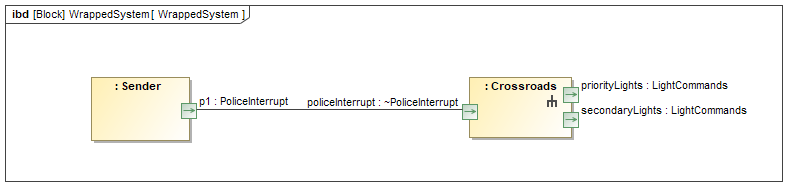
\includegraphics[width=140mm, keepaspectratio]{figures/contribution/WrappedSystem1.png}
	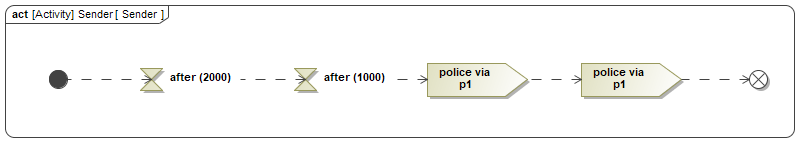
\includegraphics[width=140mm, keepaspectratio]{figures/contribution/Sender.png}
	\caption{Ellenpélda végrehajtása}
	\label{fig:activity-counter-example}
\end{figure}
Alap beállítások mellett a szimulátor nem kezeli jól az időzítéseket. Például az egyes komponensek kezdő állapotai nem a nulla időpillanatba voltak aktívak, hanem később és a különböző esemény küldések is időbe teltek amik azt eredményezték, hogy az ellenpélda nem működött a példán, hiszen a modellek nem tartalmaztak ezekre vonatkozóan információkat és a végrehajtások elcsúsztak. Szerencsére azt, hogy hogyan kezeli a szimulátor az idő múlását van lehetőség állítani \emph{Simulation Config} segítségével (\ref{fig:simconf} ábra).

A modell órájának megfelelő konfigurációja után már az ellenpéldában is szereplő időzítésekkel hajtódtak végre az állapotváltások. Ezek a \emph{start time} nullára állítása. A \emph{step delay} és \emph{step size} 1-1-re állításai voltak.
\begin{figure}[!ht]
	\centering
	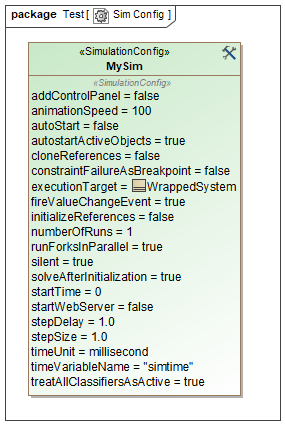
\includegraphics[width=70mm, keepaspectratio]{figures/contribution/Sim Config.png}
	\caption{Szimuláció konfigurálása}
	\label{fig:simconf}
\end{figure}
A konfigurációban az időzítéseken túl a végrehajtás más aspektusait is állítani lehet. Ami kiemelendő az a \emph{slient} mód. Ez kikapcsolja a diagramokon való animációkat. A  hivatalos dokumentáció azt ajánlja, hogy időzítés érzékeny modelleken ezt érdemes kikapcsolni. %TODO link


A szimuláció az időzítések korrekciója után sem volt működőképes. Ennek oka, hogy a szimulátor nem ugyan azon szemantika mentén hajtja végre az utasításokat, mint ami szerint a formális verifikációt elvégeztük. Például a \emph{History State} csak akkor mentette el egy állapot belső állapotait, ha az adott állapotból más állapotba lépett át a rendszer. Hurokélek esetén a végrehajtás a kezdő állapotból újraindult. Abban az esetben, ha a rendszer egy másik állapotba átlépett majd vissza a végrehajtás az elvártak szerint az utolsó aktív állapotból folytatódott.

\paragraph{Értékelés}
A szimulátort csak akkor lehet felhasználni a példák futtatása, ha a szemantika ami szerint az ellenőrzést végeztük ugyan az mint amit a szimulátor is használ. A szimulátorhoz lehetőségünk van szimulációs motort fejleszteni. Ez lehetőséget nyújthat a tulajdonságot sértő vagy alátámasztó működés végrehajtására.

\newpage
\section{Validáció}

A modellek ellenőrzése akkor lehetséges, ha a felhasználó betart bizonyos modellezési technikákat, amik lehetővé teszik a modell transzformáció végrehajtását. Ezek betartatására illetve az esetleges hibák megtalálásához készítettem egy validációs szabálykészletet. Ez olyan hibákat talál meg amik vagy ellehetetlenítik a modell transzformációját vagy olyan Gamma modellt eredményeznek ami nem lesz teljesen helyes.

\subsection{Elnevezett régiók}

\begin{tabular}{ | l | r | }
	\hline
	Név: & RegionNamedRule  \\ 
	\hline
	Azonosító: & GAMMA\_REGION\_NAMED \\
	\hline
	Súlyosság: & Error \\  
	\hline
	Üzenet: & Region must have a name \\
	\hline
\end{tabular}\newline
\newline
Erre a szabályra azért van szükség mert a \emph{Property} nyelvtanban az egyes állapotokra az őket tartalmazó régiókon keresztül lehet hivatkozni, ezért egy állapotgépen belüli el nem nevezett régiók validációs hibához vezetnek.

\subsection{Régiók nevei egyediek}

\begin{tabular}{ | l | r | }
	\hline
	Név: & RegionNameUniqueRule  \\ 
	\hline
	Azonosító: & GAMMA\_REGION\_UNIQUE \\
	\hline
	Súlyosság: & Error \\  
	\hline
	Üzenet: & Region must have a unique name \\
	\hline
\end{tabular}\newline
\newline
Szintén a fent említett hivatkozások miatt a régiók neveinek egyértelműnek kell lennie állapotgépeken belül. Az azonos nevű régiók validációs hibát dobnak.

\subsection{Szignál küldhető}

\begin{tabular}{ | l | r | }
	\hline
	Név: & SignalSendRule  \\ 
	\hline
	Azonosító: & GAMMA\_SIGNAL\_SEND \\
	\hline
	Súlyosság: & Error \\  
	\hline
	Üzenet: & Signal cannot be sent through target port \\
	\hline
\end{tabular}\newline
\newline
Ahhoz, hogy egy szignált el lehessen küldeni egy porton a port interfészén szerepelnie kell mégpedig a származtatott irányának "ki" irányúnak kell lennie. A származtatott irány nem \emph{isConjugate} esetében megegyezik a szignál interfészen feltüntetett irányával egyébként azzal ellentétes. Ez a szabály csak \emph{Send Signal} akciókra érvényes.

\subsection{Szignál fogadható}

\begin{tabular}{ | l | r | }
	\hline
	Név: & SignalReceiveRule  \\ 
	\hline
	Azonosító: & GAMMA\_SIGNAL\_RECEIVE \\
	\hline
	Súlyosság: & Error \\  
	\hline
	Üzenet: & Signal cannot be received from target port \\
	\hline
\end{tabular}\newline
\newline
Szignál fogadásához, hasonlóan mint a küldés esetében a szignálnak szerepelnie kell a megfelelő származtatott iránnyal a port interfészén. Ez a szabály \emph{Triggerek}re fut le és akkor okoz hibát, ha nem szerepel a referált szignál az interfészen vagy nem megfelelő az iránya.

\subsection{Szignál neve egyedi}
\begin{tabular}{ | l | r | }
	\hline
	Név: & SignalUniqueRule  \\ 
	\hline
	Azonosító: & GAMMA\_SIGNAL\_UNIQUE \\
	\hline
	Súlyosság: & Error \\  
	\hline
	Üzenet: & Flow property type name must be unique \\
	\hline
\end{tabular}\newline
\newline
Ahhoz, hogy szignálthoz irányt lehessen rendelni fel kell venni egy \emph{Flow Property}t és tipizálni a szignállal. A MagicDraw kikényszeríti, hogy egyedi neve legyen a \emph{Flow Property}knek az azonban lehetséges, hogy két különböző \emph{Flow Property} ugyan azt a szignált használja típusnak vagy ugyan külön szignálra hivatkoznak viszont ezek nevei megegyeznek. Ez a transzformáció során hibához vezethet hiszen a majdani \emph{Event}ek nevei ütközni fognak. Éppen ezért a \emph{Flow Property}k által használt szignálok neveinek egyedinek kell lennie.

\subsection{Kompozit blokkok}
\begin{tabular}{ | l | r | }
	\hline
	Név: & CompositeBlockRule  \\ 
	\hline
	Azonosító: & GAMMA\_COMPOSITE \\
	\hline
	Súlyosság: & Error \\  
	\hline
	Üzenet: & Composite blocks cannot define classifier behaviors \\
	\hline
\end{tabular}\newline
\newline
Blokkok vagy kompozit blokkok vagy viselkedést, állapotgépeket definiáló blokkok lehetnek. Ez a szabály hibásnak jelöl minden blokkon ami vegyesen definiál partokat és viselkedéseket.

\subsection{Statechart definíciók}
\begin{tabular}{ | l | r | }
	\hline
	Név: & StatechartBlockRule  \\ 
	\hline
	Azonosító: & GAMMA\_STATECHART \\
	\hline
	Súlyosság: & Error \\  
	\hline
	Üzenet: & Statechart blocks cannot contain parts \\
	\hline
\end{tabular}\newline
\newline
Állapotgépet definiáló blokkok nem tartalmazhatnak partokat.


